\scanpage{117}
\begin{flushright}
27 March 1968\\
17H 45\\
\end{flushright}

\begin{center}
\uline{Mister GROTHENDIECK}\\
\end{center}

\begin{enumerate}[label=\arabic*.]
\item Miss Zabardi tells me she has redone in detail 6 pages of your 17 pages of corrections. She thinks she will have finished by tomorrow evening.

\item Madam Hakim having learnt that the stencils are stored in Rue de Lille has asked Miss Chardon for 5 copies of ``Mathematical life in the Democratic Republic of Vietnam'' and proposes to run off electronic stencils.

\item We shall have the stencils of your manuscript and of Jussila's dropped off at Massy on Friday.
\end{enumerate}

\figure{\makebox[\linewidth][r]{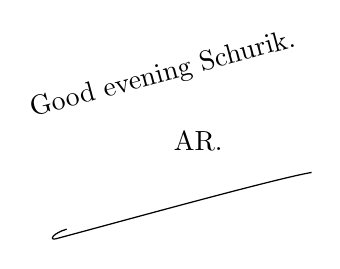
\begin{tikzpicture}[x=1em,y=1em]
\node[anchor=base west,inner sep=0,rotate=15] at (0,4.4) {\handwritten{\unsure{Good evening} Schurik.}};
\node[anchor=base west,inner sep=0] at (5.1,3.2) {\handwritten{\unsure{AR}.}};
\draw[line width=.45pt] (1.25,.35) .. controls (.75,.20) and (.60,-.05) .. (.85,0) .. controls (3.1,.60) and (8.8,2.18) .. (10.1,2.40);
\end{tikzpicture}}}
% archive sheet number: 116
